$subject$=Дополнительные главы \\ высшей математики
$date$=02.05.2025
$teacher$=Лекции Далевской О. П.

\begin{MyTheorem}
    \ThNs{Морера} $f(z)$ непрерывна в $D$ и $\forall \gamma \subset D \ \int_\gamma f(z) dz = 0 \Longrightarrow f(z)$ аналитична в $D$
\end{MyTheorem}

\begin{MyProof}
    При данных условиях $\exists \Phi(z) = \int_{z_0}^z f(\zeta) d\zeta \ | \ \Phi^\prime(z) = f(z)$ и $\Phi(z)$ аналитична

    Так как $\Phi(z)$ дифференцируема, то она дифференцируема сколько угодно раз. Таким образом, существуют $f^\prime(z), f^{\prime\prime}(z)$ и так далее, а из этого означает, что $f(z)$ -- аналитична
\end{MyProof}


\begin{MyTheorem}
    \ThNs{Лиувилля} $f(z)$ аналитична в $\Complex$ и $\exists M \in \Real^+ \ | \ |f(z)| \leq M \ \forall z \in \Complex$

    Тогда $f(z) \equiv \const$
\end{MyTheorem}


\begin{MyProof}
    Докажем, что $f^\prime(z) = 0$

    $|f^\prime(z)| = \begin{bmatrix}\text{контур } \gamma \text{ -- круг } z + \rho e^{i\varphi} \end{bmatrix} = \left|\frac{1}{2\pi i} \int_\gamma \frac{f(\zeta)}{(\zeta - z)^2} d\zeta\right| = \left|\frac{1}{2\pi i}\int_0^{2\pi} \frac{f(z + \rho e^{i \varphi}) \rho i e^{i \varphi}}{\rho ^2 e^{2 i \varphi}} d\varphi \right| \leq \frac{1}{2\pi} \int_0^{2\pi} \left| \frac{f(z + \rho e^{i \varphi})}{\rho e^{i \varphi}}\right| d\varphi \leq \frac{1}{2\pi} \int_0^{2\pi} \frac{M}{\rho} d\varphi = \frac{M}{\rho} \underset{\rho \to \infty}{\longrightarrow} 0 \Longrightarrow f(z) = \const$
    
\end{MyProof}

\Nota $w = \sin z \neq \const \Longrightarrow \sin z$ -- неограниченная функция

\subsection{4.4. Ряд Лорана}

\Def Ряд вида $\sum_{n = -\infty}^\infty C_n (z - z_0)^n$, где $C_n, z_0 \in \Complex$, называется рядом Лорана в точке $z_0$

% https://www.geogebra.org/calculator/mxctddsq

\begin{wrapfigure}[6]{R}{0pt}
    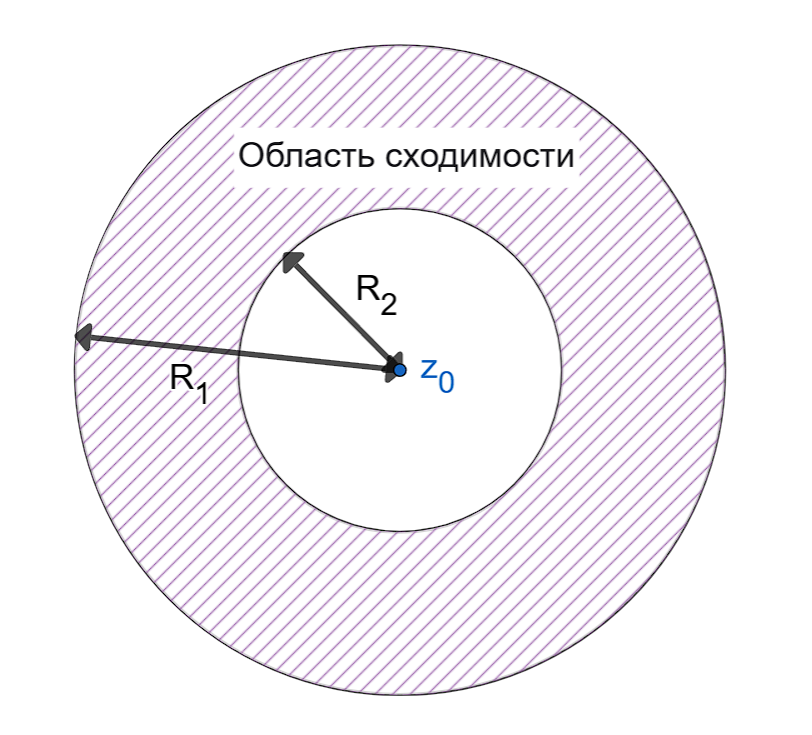
\includegraphics[width=6cm]{addchapters2/images/addchapters2_2025_05_02_1}
\end{wrapfigure}

\Nota Исследуем ряд. Обозначим $f_1 = \sum_{n = 0}^\infty C_n (z - z_0)^n$

$f_2 = \sum_{n = -1}^{-\infty} C_n (z - z_0)^n \overset{m = -n}{\Longrightarrow} \sum_{m = 1}^\infty \frac{C_{-m}}{(z - z_0)^m} = \sum_{n = 1}^\infty \frac{C_{-n}}{(z - z_0)^n}$

Тогда ряд можно записать так: $C_0 + \sum_{n = 1}^\infty \left(C_n (z - z_0)^n + \frac{C_{-n}}{(z - z_0)^n}\right)$

Рассмотрим $f_1 = \sum_{n = 0}^\infty C_n (z - z_0)^n$ -- ряд согласно теореме Абеля сходится в круге с центром $z_0$ и радиусом $R_1 = \lim_{n \to \infty} \left|\frac{C_{n}}{C_{n+1}}\right|$

Рассмотрим $f_2 = \sum_{n = 1}^\infty \frac{C_{-n}}{(z - z_0)^n} \overset{t = \frac{1}{z - z_0}}{=\joinrel=\joinrel=} \sum_{n = 1}^\infty C_{-n} t^n$ -- ряд сходится в круге $|t| < r = \lim_{n \to \infty} \left|\frac{C_{-n}}{C_{-n-1}}\right|$ или $|z - z_0| > \lim_{n \to \infty} \left|\frac{C_{-n-1}}{C_{-n}}\right| = R_2$

Таким образом, ряд Лорана сходится в \textit{кольце} с внутренним радиусом $R_2$ и внешним радиусом $R_1$ и центром $z_0$ к значению некой аналитической функции $f(z)$


\begin{MyTheorem}
    $f(z)$, аналитичная в кольце $K = (z_0, R_2, R_1)$, однозначно представима рядом Лорана в кольце $K$
\end{MyTheorem}

\begin{MyProof}
    \begin{wrapfigure}[6]{R}{5.2cm}
        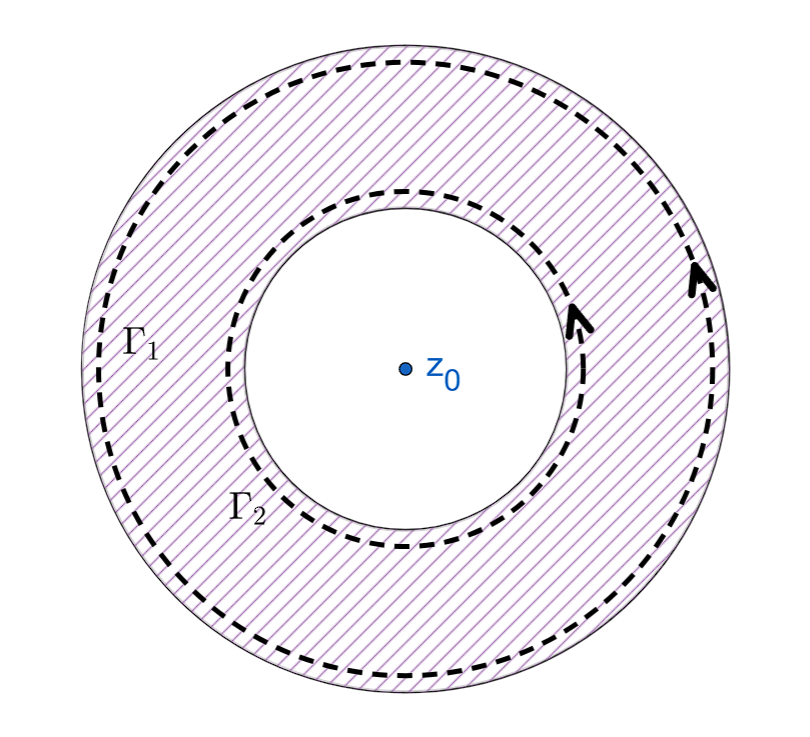
\includegraphics[width=\linewidth]{addchapters2/images/addchapters2_2025_05_02_2}
    \end{wrapfigure}

    $f(z) = \frac{1}{2\pi i} \int_\Gamma \frac{f(\zeta)}{\zeta - z} d\zeta \overset{\Gamma = \Gamma_2 \cup \Gamma_1}{=\joinrel=\joinrel=\joinrel} \frac{1}{2\pi i} \int_{\Gamma_1} \frac{f(\zeta)}{\zeta - z}d\zeta - \frac{1}{2\pi i} \int_{\Gamma_2} \frac{f(\zeta)}{\zeta - z} d\zeta$

    Разложим $\frac{1}{\zeta - z}$ в ряд Тейлора:

    $\frac{1}{\zeta - z} = \frac{1}{\zeta - z_0 - (z - z_0)} = 
    \begin{sqcases}
        \frac{1}{(\zeta - z_0)(1 - (\frac{z - z_0}{\zeta - z_0}))} = \sum_{n = 1}^\infty \frac{(z - z_0)^n}{(\zeta - z_0)^{n + 1}}\\ 
        \frac{1}{-(z - z_0)(1 - (\frac{\zeta - z_0}{z - z_0}))} = -\sum_{n = 1}^\infty \frac{(\zeta - z_0)^n}{(z - z_0)^{n + 1}}
    \end{sqcases}$

    1. Первый ряд сходится, если $\frac{z - z_0}{\zeta - z_0} < 1 \Longleftrightarrow |z - z_0| < |\zeta - z_0|$ -- это $\Gamma_1$

    Также $\frac{f(\zeta)}{\zeta - z} = \sum_{n = 0}^\infty \frac{f(\zeta)(z - z_0)^n}{(\zeta - z_0)^{n + 1}}$

    По теореме Коши:

    $f(z) = \frac{1}{2\pi i} \int_{\Gamma_1} \frac{f(\zeta)}{\zeta - z} d\zeta = \frac{1}{2\pi i} \sum_{n = 0}^\infty \left(\int_{\Gamma_1} \frac{f(\zeta)d\zeta}{(\zeta - z_0)^{n + 1}}\right) (z - z_0)^n = \sum_{n = 0}^\infty C_n (z - z_0)^n$

    Из этого $C_n = \frac{1}{2\pi i} \int_{\Gamma_1} \frac{f(\zeta)d\zeta}{(\zeta - z_0)^{n + 1}}$ \\

    2. Второй ряд сходится, если $\frac{z - z_0}{\zeta - z_0} < 1 \Longleftrightarrow |z - z_0| > |\zeta - z_0|$ -- это $\Gamma_2$

    \Lab
\end{MyProof}

\Nota Таким образом, коэффициенты ряда Лорана $C_n = \frac{1}{2\pi i} \int_{\Gamma_i} \frac{f(\zeta)}{(\zeta - z_0)^{n + 1}} d\zeta$

\Def Изолированной особой точкой однозначного характера называется точка $a \in \Complex \ | \ f(z)$ аналитична в кольце $0 < |z - a| < \rho$, но не определена в $z = a$

\Defs Точка $a = \infty$ называется изолированной особой, если $f(z)$ аналитична в кольце $\rho < |z| < \infty$

\Defs Устранимой особой точкой $a$ называется точка, для которой $\lim_{z \to a} f(z) \in \Complex$, в $a$ функция не определена

Полюсом $a$ называется точка, для которой $\lim_{z \to a} f(z) = \infty$

Существенно особой точкой $a$ называется точка, для которой $\nexists \lim_{z \to a} f(z)$

\ExN{1} Для $f(z) = \frac{\sin z}{z}$ точка $z = 0$ является устранимой особой -- $\lim_{z \to 0} \frac{\sin z}{z} = 1$

\ExNs{2} Для $f(z) = \frac{z}{(z + i)^2} \quad \lim_{z \to -i} \frac{z}{(z + i)^2} = \left[\frac{1}{0^2} = \infty^2\right]$, $a = -i$ - полюс 2-ого порядка

\ExNs{3} Для $f(z) = \sin z \quad \nexists \lim_{z \to \infty} \sin z$ 

\Def Для ряда Лорана функции $f(z)$ в окрестности особой точки $z = a \in \Complex \quad f(z) = \underset{\text{это правильная часть}}{\underbrace{\sum_{n = 0}^\infty C_n (z - a)^n}} + \underset{\text{это главная часть}}{\underbrace{\sum_{n = 1}^\infty \frac{C_{-n}}{(z - a)^n}}}$

\Def Для ряда Лорана в $a = \infty$: $f(z) = \sum_{n = -\infty}^\infty C_n z^n = \underset{\text{это главная часть}}{\underbrace{\sum_{n = 1}^\infty C_n z^n}} + \underset{\text{это правильная часть}}{\underbrace{\sum_{n = 0}^\infty \frac{C_{-n}}{z^n}}}$

\Def Вычетом $\residuum(f(z), z_0)$ функции $f(z)$ в точке $z_0$ называется $C_{-1}$ коэффициент ряда Лорана, если $z_0 \in \Complex$, и $-C_{-1}$, если $z_0 = \infty$


